\RequirePackage{luatex85}
\documentclass{article}
\usepackage{tikz}
\usepackage[letterpaper, margin=0in, top=0.34in]{geometry}
\usepackage{expl3}
\ExplSyntaxOn
\cs_new_eq:NN \Repeat \prg_replicate:nn
\ExplSyntaxOff

\begin{document}
\LARGE\sf\centering
\Repeat{2}{\noindent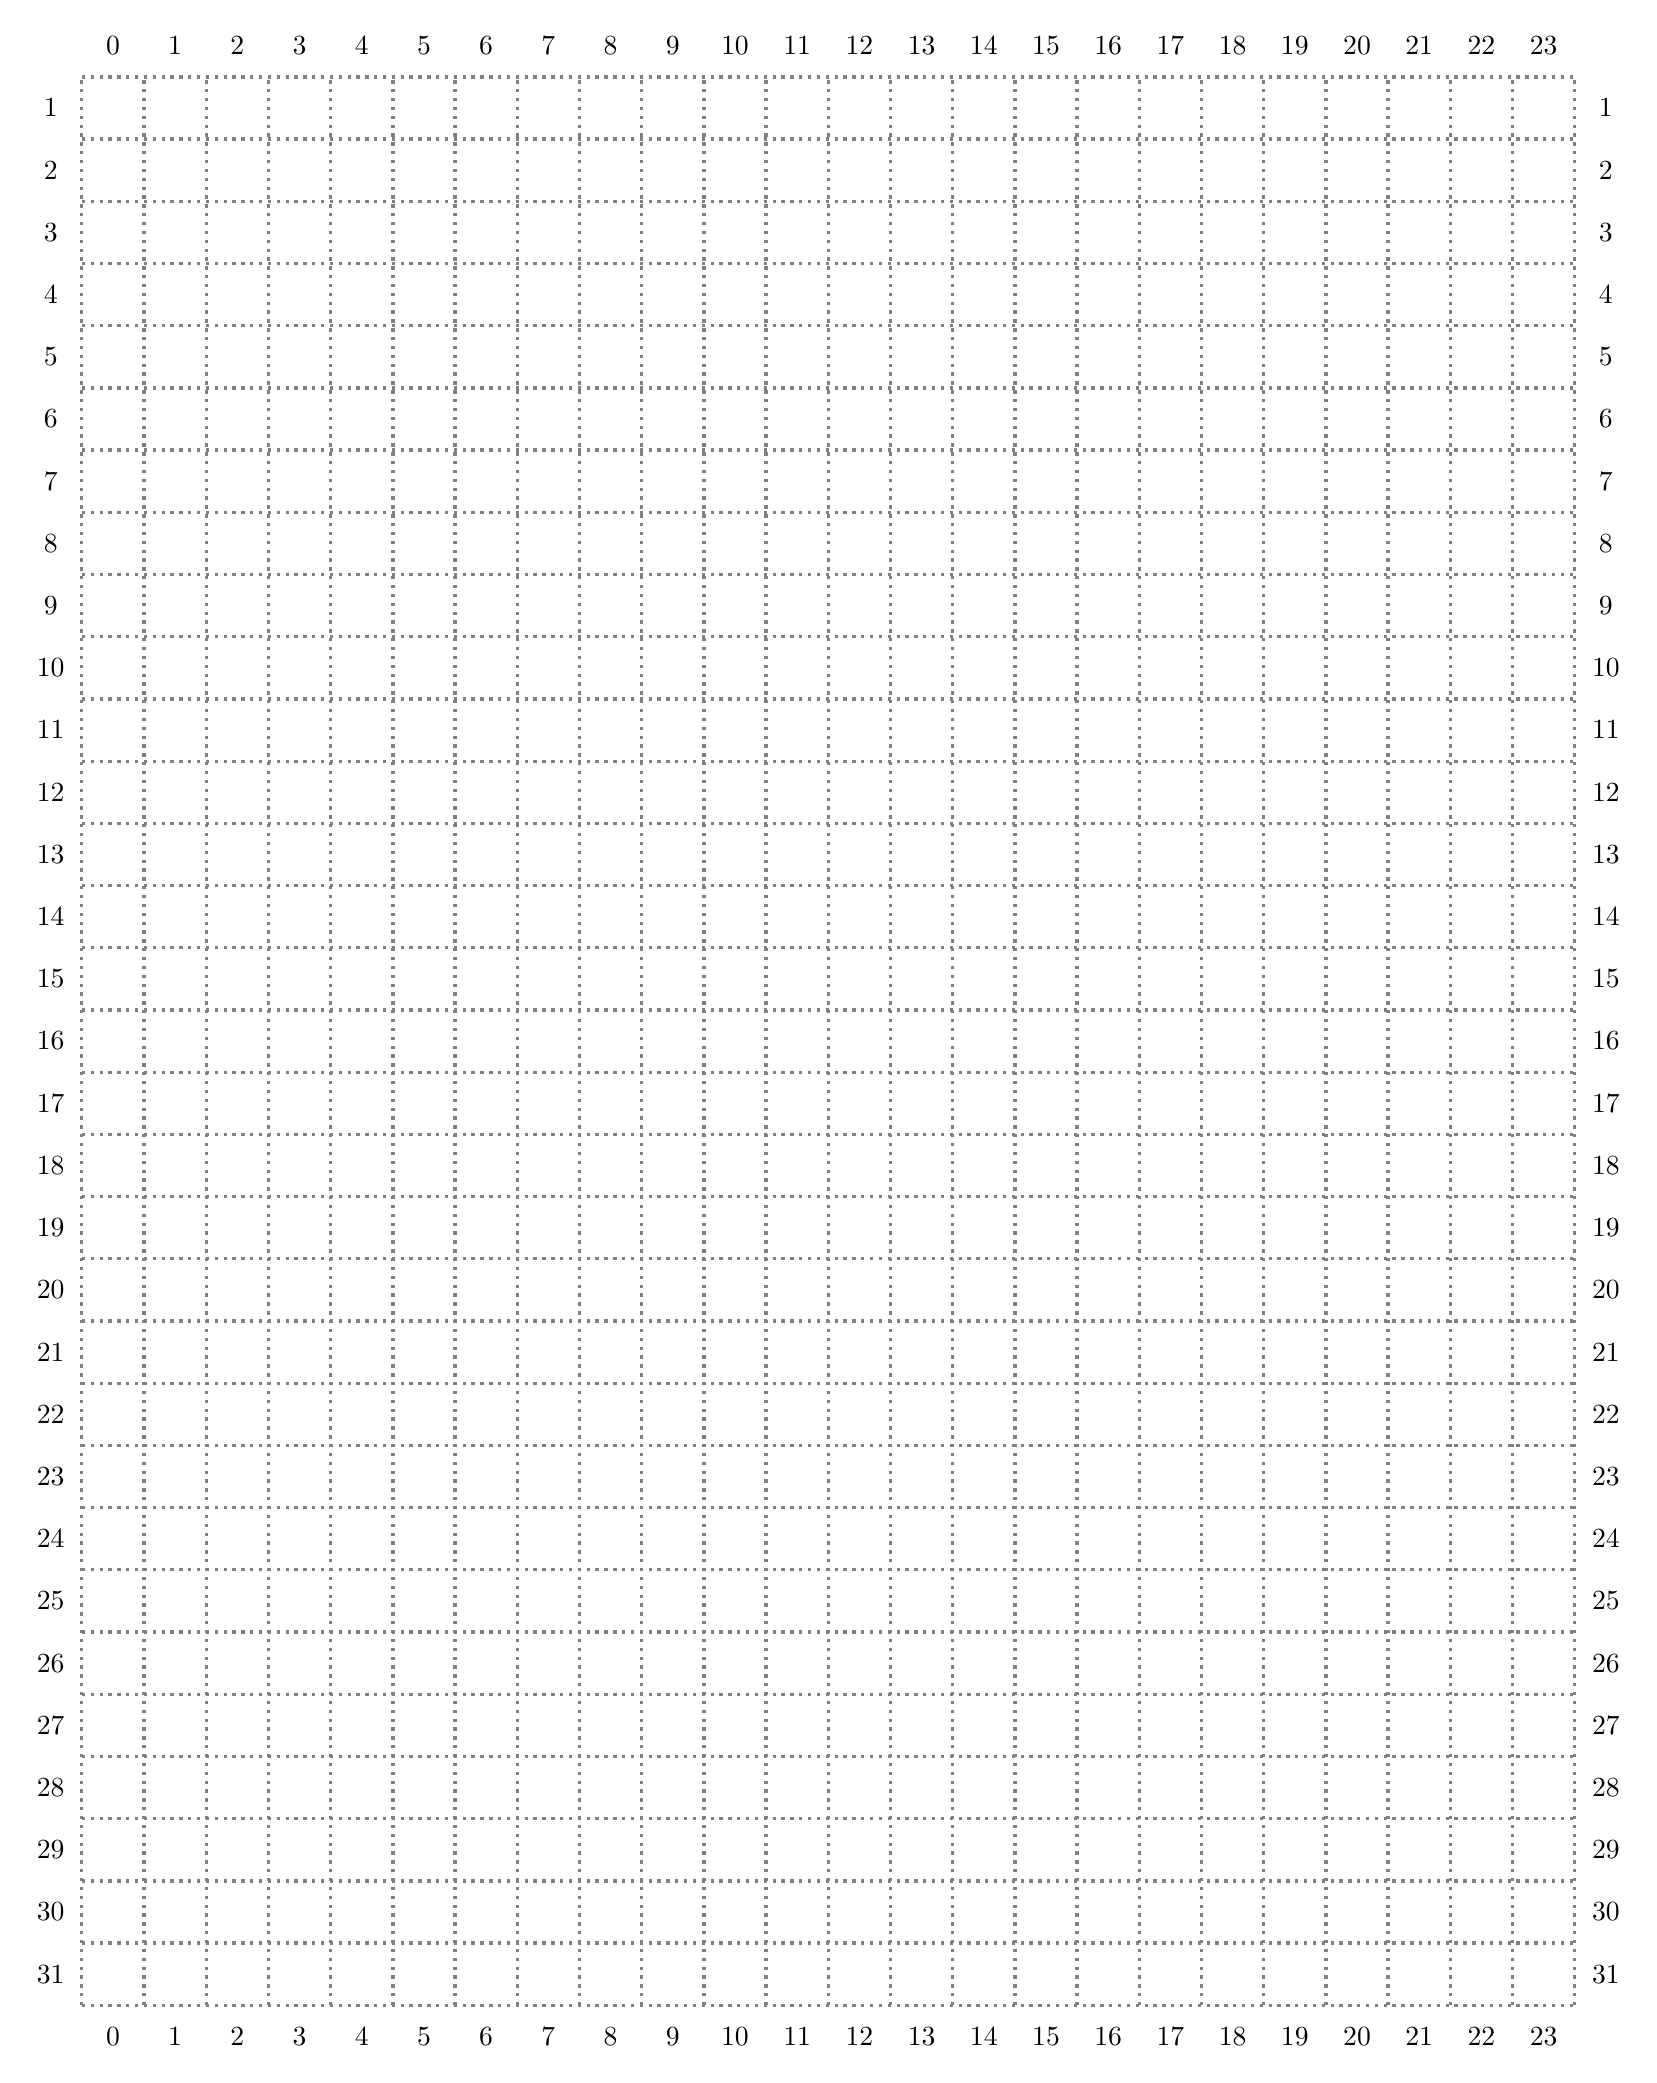
\begin{tikzpicture}
	[scale=0.79, very thick, dotted]
	\draw[gray] (0,0) grid (24,-31);
	\foreach \x in {0,...,23}
	{	\draw (\x+0.5, 0.5) node {\x};
		\draw (\x+0.5, -31.5) node {\x};
		}
	\foreach \y in {1,...,31}
	{	\draw (-0.5,0.5-\y) node {\y};
		\draw (24.5,0.5-\y) node {\y};
		}
	\end{tikzpicture}\par}
\end{document}